% !TEX root = ../Preparazione alle olimpiadi.tex

\chapter{Brute Force e Algoritmi Greedy}


In questo capitolo analizzeremo due approcci fondamentali alla risoluzione dei problemi: 
gli algoritmi \textbf{Brute Force} e gli algoritmi \textbf{Greedy}.  
Si tratta di due paradigmi concettualmente semplici, ma molto diversi tra loro per strategia, 
prestazioni e casi d’uso.

Il \textbf{Brute Force} adotta un approccio esaustivo: esplora tutte le soluzioni possibili 
e seleziona quella corretta o quella ottimale. È un metodo semplice, intuitivo e sempre corretto, 
ma spesso troppo lento per input di dimensioni elevate.

Gli algoritmi \textbf{Greedy}, al contrario, seguono una strategia “miope”: 
a ogni passo scelgono la soluzione che sembra migliore in quel momento, 
senza considerare le conseguenze future.  
Questo permette grande efficienza, ma non garantisce sempre una soluzione ottimale.

\section{Algoritmi Brute Force}

Gli algoritmi Brute Force rappresentano il metodo più semplice e diretto per risolvere un problema: 
consistono nel generare e valutare \textbf{tutte} le soluzioni possibili, scegliendo poi quella corretta 
o quella ottimale. Questo approccio è intuitivo e non richiede strutture dati o strategie sofisticate: 
si limita a esplorare in maniera esaustiva l’intero spazio delle soluzioni.

La forza del metodo Brute Force risiede nella sua semplicità: poiché vengono considerate tutte le possibilità, 
l’algoritmo garantisce sempre la correttezza della soluzione trovata. Tuttavia, la sua debolezza è altrettanto 
evidente: il numero di combinazioni cresce spesso in modo \textbf{esponenziale}, rendendo il Brute Force 
impraticabile per problemi di dimensioni medio-grandi.

Nonostante ciò, gli algoritmi Brute Force sono fondamentali per diversi motivi:
\begin{itemize}
	\item sono facili da implementare e utili come punto di partenza;
	\item forniscono una soluzione ottima, quando è possibile enumerare tutto lo spazio delle soluzioni;
	\item permettono di confrontare la qualità di algoritmi più avanzati;
	\item sono spesso accettabili quando i dati in input sono piccoli oppure quando il problema non richiede 
	una soluzione immediata.
\end{itemize}








\newpage
\subsection{Antivirus}
\href{https://territoriali.olinfo.it/task/antivirus}{Link al problema} 

\smallskip

\noindent Time limit = 1.00s, Memory limit = 512 MB

\bigskip

Il nuovo sistema di gara delle Selezioni Territoriali funziona alla grande, ma sembra che la mascotte abbia fiutato un virus nascosto fra i file inviati da un partecipante!  
Conosciamo la lunghezza del virus e sappiamo che si ripete uguale nei quattro file ricevuti, ma non sappiamo dove. Aiutaci a individuare il virus!

\medskip

\noindent\textbf{Dettagli:}

 Sono dati in input quattro file \(F_1, F_2, F_3, F_4\), rappresentati come quattro stringhe di caratteri di lunghezza rispettivamente \(N_1, N_2, N_3, N_4\).  

Il virus è una stringa \(V\) di lunghezza \(M\). La lunghezza \(M\) è nota (viene fornita in input), ma non conosciamo il contenuto della stringa \(V\) del virus.  
Sappiamo con certezza che \(V\) appare all'interno di tutti e quattro i file, come sottostringa di caratteri \emph{consecutivi}. Sappiamo inoltre che \emph{NON} ci sono altre sottostringhe consecutive di lunghezza \(M\) che si ripetono uguali in tutti e quattro i file.


Le posizioni dei caratteri nelle stringhe sono numerati a partire da \(0\). Per ciascuno dei quattro file \(F_i\), trova la posizione in cui è inserito il virus, ovvero la posizione dove appare il primo carattere del virus \(V\) all'interno della stringa \(F_i\)

L’obiettivo è: per ciascuno dei quattro file \(F_i\), trovare la posizione (indice, a partire da 0) in cui compare \(V\), ovvero l’indice del primo carattere di \(V\) dentro \(F_i\).

\bigskip

\noindent\textbf{Formato di input}  

La prima riga contiene un intero \(T\), il numero di casi di test.  
Seguono \(T\) casi di test, ognuno preceduto da una riga vuota.  

Per ciascun caso di test:
\begin{itemize}
	\item Una riga con quattro interi \(N_1, N_2, N_3, N_4\) — le lunghezze dei quattro file.
	\item Una riga con un intero \(M\) — la lunghezza del virus.
	\item Quattro righe contenenti le stringhe \(F_1, F_2, F_3, F_4\).
\end{itemize}

\bigskip

\noindent\textbf{Formato di output}  

Per ogni caso di test, stampare:
\[
\texttt{Case \#t:}\; p_1\; p_2\; p_3\; p_4
\]
dove \(t\) è il numero del caso (a partire da 1), e \(p_i\) è la posizione (indice 0‑based) della prima occorrenza della stringa virus \(V\) dentro \(F_i\).

\bigskip

\noindent\textbf{Assunzioni e Vincoli}  


\begin{itemize}
	
\item $T = 12$

\item $2 \le N_1, N_2, N_3, N_4 \le 100$

\item $2 \le M \le 20$

\item $M \le \min(N_1, N_2, N_3, N_4)$



	\item Tutti i caratteri dei file sono lettere minuscole dell'alfabeto inflese (dalla a alla z), NON sono presenti spazi.


	\item È garantito che il virus esiste ed è unico
	
\end{itemize}



\newpage

\noindent\textbf{Esempio}  

\smallskip  
\textbf{Input:}  
\begin{verbatim}
	2
	
	8 12 10 7
	4
	ananasso
	associazione
	tassonomia
	massone
	
	6 9 11 10
	3
	simone
	ponessimo
	milionesimo
	cassonetto
\end{verbatim}

\smallskip  
\textbf{Output:}  
\begin{verbatim}
	Case #1: 4 0 1 1
	Case #2: 3 1 4 4
\end{verbatim}

\noindent\textbf{Spiegazione:} 

Nel primo caso il virus è “asso”: anan\textbf{asso}, \textbf{asso}ciazione, t\textbf{asso}nomia, m\textbf{asso}ne.

Nel secondo caso il virus è “one”: sim\textbf{one}, p\textbf{one}ssimo, mili\textbf{one}simo, cass\textbf{one}tto.


\bigskip

\noindent \textbf{Idea (brute force)}: 

Si considerano tutte le possibili sottostringhe di lunghezza \(M\) della prima stringa \(F_1\).
Ogni sottostringa di questo tipo costituisce una possibile candidata a essere il virus.

Per ciascuna sottostringa candidata:
\begin{itemize}
	\item si verifica se essa compare almeno una volta nella stringa \(F_2\);
	\item si verifica se essa compare almeno una volta nella stringa \(F_3\);
	\item si verifica se essa compare almeno una volta nella stringa \(F_4\).
\end{itemize}

Il controllo viene effettuato confrontando la sottostringa candidata con tutte le sottostringhe
di lunghezza \(M\) delle altre stringhe.

Appena una sottostringa candidata risulta presente in tutte e quattro le stringhe,
essa è necessariamente il virus, poiché il problema ne garantisce l’esistenza e l’unicità;
a questo punto l’algoritmo può terminare.

Infine, si memorizzano le posizioni in cui il virus compare all’interno di ciascuna stringa.

\newpage

\noindent \textbf{Implementazione C++ - Brute Force}


\begin{lstlisting}[language=C++]
	#include <bits/stdc++.h>  
	using namespace std;
	
	int main()
	{
		// Apro il file di input
		ifstream inputFile("antivirus_input_1.txt");
		
		int T;                  // Numero di test case nel file
		inputFile >> T;
		
		// Ciclo su tutti i test case
		for (int test = 1; test <= T; ++test)
		{
			// N1, N2, N3, N4 sono le lunghezze delle quattro stringhe F1, F2, F3, F4
			int N1, N2, N3, N4;
			inputFile >> N1 >> N2 >> N3 >> N4;
			
			// M è la lunghezza della sottostringa del virus
			int M;
			inputFile >> M;
			
			// Le quattro stringhe in cui cercare il virus
			string F1, F2, F3, F4;
			inputFile >> F1 >> F2 >> F3 >> F4;
			
			// Variabili per salvare la posizione in cui il virus appare in ciascuna stringa
			int F1_virus;  // Posizione in F1 da cui inizia la sottostringa candidata
			int F2_virus;  // Posizione in F2 dove compare la sottostringa candidata
			int F3_virus;  // Posizione in F3 dove compare la sottostringa candidata
			int F4_virus;  // Posizione in F4 dove compare la sottostringa candidata
			
			/*
			Ciclo principale: scorriamo tutte le sottostringhe di lunghezza M in F1
			e le consideriamo candidate al virus
			*/
			for(int i = 0; i <= F1.length(); i++){
				F1_virus = i;    // La sottostringa candidata parte da posizione i in F1
				F2_virus = -1;   // Inizializzo a -1, se rimane -1 vuol dire che non l'ho trovata
				F3_virus = -1;
				F4_virus = -1;
				
				// Estraggo la sottostringa candidata dalla stringa F1
				string virus_candidato = F1.substr(i, M);
				
				// Cerco il virus in F2
				for(int j = 0; j < F2.length(); j++){
					if(F2.substr(j, M) == virus_candidato){  // confronto ogni sottostringa di F2
						F2_virus = j;  // trovato, salvo la posizione
						break;         // esco dal ciclo
					}
				}
				
				// Cerco il virus in F3
				for(int j = 0; j < F3.length(); j++){
					if(F3.substr(j, M) == virus_candidato){
						F3_virus = j;
						break;
					}
				}
				
				// Cerco il virus in F4
				for(int j = 0; j < F4.length(); j++){
					if(F4.substr(j, M) == virus_candidato){
						F4_virus = j;
						break;
					}
				}
				
				// Se la sottostringa candidata e' presente in tutte e quattro le stringhe, abbiamo trovato il virus
				if(F2_virus != -1 && F3_virus != -1 && F4_virus != -1){
					break;  // esco dal ciclo su F1
				}
			}
			
			// Stampo le posizioni trovate per ciascuna stringa
			cout << "Case #" << test << ": " 
			<< F1_virus << " " 
			<< F2_virus << " " 
			<< F3_virus << " " 
			<< F4_virus << endl;
		}
		
		inputFile.close();  // Chiudo il file di input
		return 0;
	}
	
\end{lstlisting}

\bigskip
\noindent \textbf{Costo Computazionale}: \\

Il costo computazionale è:
\begin{itemize}
	\item $O(N_2) + O(N_3) + O(N_4)$ per i cicli interni nelle righe 47, 55, 63;
	\item $O(N_1)$ per il ciclo esterno alla riga 37.
\end{itemize}

Ciò significa che i cicli più interni vengono eseguiti $N_1$ volte.

La complessità totale è quindi: 
\begin{align*}
	&= O(N_1) \cdot [O(N_2) + O(N_3) + O(N_4)] \\
	&\approx O(N_1) \cdot \max(O(N_2), O(N_3), O(N_4))
\end{align*}

Dai vincoli del problema:
\[
2 \le N_i \le 100
\]

la complessità può essere stimata come: 
\begin{align*}
	&\approx O(N_1) \cdot O(100) \\
	&\approx O(100 \cdot 100) \\
	&= O(10^4)
\end{align*}

Pertanto, considerando una macchina che esegue circa $10^8$ operazioni al secondo, il tempo stimato di esecuzione sarebbe:
\[
\frac{10^4}{10^8} \text{ secondi } = 10^{-4} \text{ secondi.}
\]

\noindent
In conclusione, il programma è coerente con il limite di tempo imposto dal problema (1.00 s).


L’approccio \emph{brute force} è, in generale, il più dispendioso dal punto di vista computazionale.
In questo caso specifico, tuttavia, la dimensione ridotta degli input consente di rientrare nei limiti temporali previsti, permettendo al programma di terminare correttamente l’esecuzione.

Nella maggior parte dei casi, però, tale strategia non è applicabile e si rende necessario ricorrere a metodi algoritmici più efficienti.

Di seguito vengono presentati due problemi risolti mediante un approccio \emph{brute force} che, nonostante la correttezza logica della soluzione, non rispettano i vincoli temporali imposti dal problema.







\newpage

\subsection{Apple Division}
\href{https://cses.fi/problemset/task/1623/}{Link al problema}

\smallskip

\noindent Time limit = 1.00s, Memory limit = 512 MB

\bigskip

There are n apples with known weights. Your task is to divide the apples into two groups so that the difference between the weights of the groups is minimal.


\bigskip

\noindent\textbf{Input}

The first input line has an integer $n$: the number of apples.
The next line has $n$ integers $p_1,p_2,\dots,p_n$: the weight of each apple.

\bigskip

\noindent\textbf{Output}

Print one integer: the minimum difference between the weights of the groups.

\bigskip

\noindent\textbf{Constraints}

\begin{itemize}
	\item \(1 \le n \le 20\)
	\item \(1 \le p_i \le 10^9\)
\end{itemize}


\noindent\textbf{Example}

\smallskip
\textbf{Input:}
\begin{verbatim}
	5
	3 2 7 4 1
\end{verbatim}

\smallskip
\textbf{Output:}
\begin{verbatim}
	1
\end{verbatim}

\smallskip
Explanation: Group 1 has weights 2, 3 and 4 (total weight 9), and group 2 has weights 1 and 7 (total weight 8).

\bigskip
\noindent \textbf{Idea (brute force):}

si associa alle \(N\) mele un array binario di lunghezza \(N\), comunemente chiamato \emph{bit mask}, che viene incrementato di \(1\) a ogni iterazione.  
In questo modo la bit mask assume, in successione, tutti i possibili valori binari:

\medskip
\noindent$000001$ \\
$000010$ \\
$000011$ \\
$000100$ \\
$000101$ \\
\dots \\
$111111$
\medskip

Ogni configurazione rappresenta una possibile suddivisione delle mele in due gruppi:  
se il bit in posizione \(i\) vale \(1\), la mela \(i\)-esima viene assegnata al primo gruppo;  
se vale \(0\), viene assegnata al secondo gruppo.

Scorrendo tutte le possibili bit mask, si esplorano tutte le combinazioni possibili di suddivisione delle mele.  
Per ciascuna configurazione si calcola la differenza tra la somma dei pesi dei due gruppi, scegliendo infine quella che minimizza tale differenza.




\newpage
\noindent	\textbf{Implementazione C++ - Brute Force:}

\begin{lstlisting}[language=C++]
#include <bits/stdc++.h>
using namespace std;

// Funzione che calcola la somma dei pesi delle mele selezionate dalla bit mask apple_bit
int64_t somma_apple(int N, vector<bool> apple_bit, vector<int64_t> &apples)
{
	// Variabile che conterra' la somma dei pesi selezionati
	int64_t somma = 0;
	
	// Scorre tutte le N mele
	for (int i = 0; i < N; i++)
	{
		// Se il bit i-esimo è a 1, la mela i-esima viene selezionata
		if (apple_bit[i])
		{
			// Aggiunge il peso della mela alla somma
			somma += apples[i];
		}
	}
	// Ritorna la somma dei pesi del gruppo selezionato
	return somma;
}

int main()
{
	// Numero di mele
	int N;
	cin >> N;
	
	// Vettore che contiene i pesi delle mele
	vector<int64_t> apples;
	
	// Bit mask inizializzata a tutti 0 (nessuna mela selezionata)
	vector<bool> apple_bit(N, 0);
	
	// Somma totale dei pesi di tutte le mele
	int64_t somma_tot = 0;
	
	// Somma del gruppo selezionato dalla bit mask corrente
	int64_t somma_provvisoria = 0;
	
	// Differenza minima trovata (inizializzata a un valore molto grande)
	int64_t diff = INT_MAX;
	
	// Lettura dei pesi delle mele
	for (int i = 0; i < N; i++)
	{
		int64_t apple;
		cin >> apple;
		
		// Inserisce il peso nel vettore
		apples.push_back(apple);
	}
	
	// Calcolo della somma totale dei pesi
	for (int apple : apples)
	{
		somma_tot += apple;
	}
	
	// Ciclo che simula l'incremento della bit mask
	// e prova tutte le possibili combinazioni
	
	//il while va avanti fin quando la somma di tutti i pesi delle mele non coincide con la somma totale. In pratica, va avanti fin quando la bit_mask non raggiunge il valore corrispondente a N 1
	while (somma_provvisoria < somma_tot)
	{
		// Simula l'incremento binario della bit mask
		for (int i = N - 1; i >= 0; i--)
		{
			// Se il bit è 0, lo porta a 1 e si ferma
			if (apple_bit[i] == 0)
			{
				apple_bit[i] = 1;
				
				// Calcola la somma del gruppo selezionato
				somma_provvisoria = somma_apple(N, apple_bit, apples);
				
				// Calcola la differenza tra i due gruppi
				// (somma_tot - somma_provvisoria) è il peso del secondo gruppo
				diff = min(diff, abs(somma_tot - somma_provvisoria - somma_provvisoria));
				
				// Interrompe il ciclo perché l'incremento è completato
				break;
			}
			else
			{
				// Se il bit è 1, lo riporta a 0 (riporto binario)
				apple_bit[i] = 0;
			}
		}
	}
	
	// Stampa la minima differenza trovata
	cout << diff << endl;
	
	return 0;
}

\end{lstlisting}



\bigskip
\noindent \textbf{Costo Computazionale}: \\
Il costo computazionale è:
\begin{itemize}
	\item $O(n)$ per il ciclo for alla riga 56, che calcola la somma dei pesi delle $N$ mele
	\item $O(n)$ per la funzione \texttt{somma\_apple}, che scorre tutte le $n$ mele alla riga 11.
	\item $O(2^n)$ per il ciclo che genera tutte le possibili bit mask (riga 65)
\end{itemize}

La complessità è:
\begin{align*}
	&= O(n) + O(2^n) \cdot O(n) \\
	&= O(2^n \cdot n)
\end{align*}

dove:
\begin{itemize}
	\item $n$ è il numero di mele
\end{itemize}

\bigskip
Dai vincoli del problema:
\[
1 \le n \le 20
\]

il numero massimo di combinazioni da esplorare è:
\[
2^{20} = 1\,048\,576
\]

Sostituendo nella complessità, otteniamo:
\[
O(2^n \cdot n) = O(2^{20} \cdot 20) \approx O(2 \cdot 10^7)
\]

Considerando una macchina che esegue circa \(10^8\) operazioni al secondo, il tempo stimato di esecuzione è:
\[
\frac{2 \cdot 10^7}{10^8} = 0.2 \text{ secondi}
\]

\noindent
Pertanto, questo approccio brute force risulta accettabile per i vincoli del problema e rientra nel time limit di 1 secondo.





\newpage


\subsection{Stick Lengths}
\label{problema:brute-force:Sticks-Length}
\href{https://cses.fi/alon/task/1074}{Link al problema} 

\smallskip

\noindent Time limit = 1.00s, Memory limit = 512 MB

\bigskip

	
	There are $n$ sticks with some lengths. Your task is to modify the sticks so that each stick has the same length.
	\medskip
	
	You can either lengthen and shorten each stick. Both operations cost $x$ where $x$ is the difference between the new and original length.
	\medskip
	
	What is the minimum total cost?
		
		\bigskip
		
		\noindent	\textbf{Input:} 
		
		The first input line contains an integer $n$: the number of sticks.
		
		\medskip  
	Then there are $n$ integers: \(p_1, p_2, \ldots, p_n\): the lengths of the sticks.
	
	
		
		\bigskip
		
		\noindent \textbf{Output:}  
		
	Print one integer: the minimum total cost.
		
		\bigskip
		
		\noindent \textbf{Constraints:}
		
		
		\begin{aligned}
			1 &\le n \le 2 \cdot 10^{5} \\
			1 &\le p_i \le 10^{9} 
		\end{aligned}
		
	 
		
		
		\bigskip
		
		\noindent \textbf{Example:}
		\begin{verbatim}
			Input:
			5
			2 3 1 5 2
			
			Output:
			5
		\end{verbatim}
		
		\noindent \textbf{Idea (brute force)}:
		
		provare ogni possibile scelta di lunghezza target tra quelle presenti nei dati e calcolare il costo totale per uniformare tutti i bastoncini a quel valore; quindi scegliere il minimo tra tutti i costi calcolati.
		Nel caso d'esempio d'input, occorre calcolare quanto costa uniformare tutti i numeri a 1, poi a 2, poi a 3, poi a 4 ed infine a 5
		
	
	\bigskip
		
	\noindent	\textbf{Implementazione C++ - Brute Force:}
		
		\begin{lstlisting}[language=C++]
#include <bits/stdc++.h>
using namespace std;

int main()
{
	vector<int> sticks;           // Vettore che conterra' le lunghezze dei bastoncini
	int numbers;                  // Numero di bastoncini n
	int costo_minimo = INT_MAX;   // Variabile per memorizzare il costo minimo trovato, inizializzata all'infinito
	
	cin >> numbers;               // Leggo n, il numero di bastoncini
	
	// Ciclo per leggere le lunghezze dei bastoncini: O(n)
	for (int i = 0; i < numbers; i++)
	{
		int stick;
		cin >> stick;             // Leggo la lunghezza di un bastoncino
		sticks.push_back(stick);  // Inserisco la lunghezza nel vettore
	}
	
	// Calcolo il minimo e il massimo tra le lunghezze: O(n)
	int minimo = *min_element(sticks.begin(), sticks.end());
	int massimo = *max_element(sticks.begin(), sticks.end());
	
	// Ciclo principale: provo ogni possibile lunghezza target tra minimo e massimo
	// Complessita': O(R * n), dove R = massimo - minimo
	for (int i = minimo; i <= massimo; i++)
	{
		int somma_costi = 0; // Somma dei costi per portare tutti i bastoncini alla lunghezza target i
		
		// Per ogni bastoncino calcolo il costo per portarlo alla lunghezza target i: O(n)
		for (int stick : sticks)
		{
			int costo = abs(stick - i);  // Differenza tra lunghezza attuale e target
			somma_costi += costo;        // Aggiungo il costo totale
		}
		
		// Aggiorno il costo minimo se la somma dei costi corrente è inferiore
		costo_minimo = min(costo_minimo, somma_costi);
	}
	
	cout << costo_minimo;  // Stampo il costo totale minimo
	
	return 0;
}

	\end{lstlisting}
	
	\bigskip
	\noindent \textbf{Costo Computazionale}: \\
	Il costo computazionale è:
	\begin{itemize}
		\item $O(n)$ per il for della riga 13
		\item $O(n)$ per la funzione $min\_element$ della riga 21
		\item $O(n)$ per la funzione $max\_element$ della riga 22
		\item $O(massimo - minimo) \cdot O(n) $ per il for della riga 26 (includendo l'interno)
	\end{itemize}
	
	La complessità è: 
\begin{align*}
	&= O(n) + O(n) + O(n) + O(\text{massimo} - \text{minimo}) \cdot O(n) \\
	&= O(n) + O(R \cdot n) \\
	&= O(R \cdot n)
\end{align*}
	dove: $R =$ massimo - minimo, $n = $ numero di bastoncini
	

	Dai vincoli del problema:
	
	\[
	1 \le n \le 2 \cdot 10^5, \quad 1 \le p_i \le 10^9,
	\]
	
	quindi il valore massimo di \(R\) può arrivare fino a
	
	\[
	R \le 10^9.
	\]
	
	Sostituendo nella complessità, otteniamo:
	
	\[
	O(R \cdot n) = O(10^9 \cdot 2 \cdot 10^5) = O(2 \cdot 10^{14}).
	\]
	
	Considerando una macchina che esegue circa \(10^8\) operazioni al secondo, il tempo stimato di esecuzione sarebbe:
	
	\[
	\frac{2 \cdot 10^{14}}{10^8} = 2 \cdot 10^6 \text{ secondi } \approx 23 \text{ giorni!}
	\]
	
	\noindent
	Pertanto, questo approccio è praticamente inefficiente e supera di gran lunga il time limit di 1 secondo. 
	
	Per risolvere il problema in tempo ragionevole, è 
	necessario un algoritmo più efficiente, ad esempio basato sulla mediana dei bastoncini che vedremo in seguito.
	
	
	
	

	\newpage
	
	
	\subsection{Nearest Smaller Values}
	\label{problema:brute-force:Nearest-Smaller-Values}
	
	\href{https://cses.fi/alon/task/1645/}{Link al problema} 
	
	\smallskip
	
	\noindent Time limit = 1.00s, Memory limit = 512 MB
	
	\bigskip
	
	Given an array of n integers, your task is to find for each array position the nearest position to its left having a smaller value.
	
	\bigskip
	
	\noindent \textbf{Input:}
	The first input line has an integer n: the size of the array.
	The second line has n integers $x_1,x_2,\dots,x_n$: the array values.
	
	\bigskip
	\noindent \textbf{Output:}
	Print $n$ integers: for each array position the nearest position with a smaller value. If there is no such position, print 0.
	
	\bigskip
	
	\noindent \textbf{Constraints: } \\
	\begin{equation*}
		1 \le n \le 2 \cdot 10^5
	\end{equation*}
	
	\begin{equation*}
		1 \le x_i \le 10^9
	\end{equation*}
	
	\bigskip
	
	\noindent \textbf{Example:} 
	
	\begin{verbatim}
		Input: 
		8
		2 5 1 4 8 3 2 5
	\end{verbatim}
	
		
	\begin{verbatim}
		Output: 
		0 1 0 3 4 3 3 7
	\end{verbatim}
	
	\bigskip
	
	\noindent \textbf{Idea (brute force)}: 
	Dato un array di $N$ numeri interi, per ogni posizione $i$ si vogliono analizzare tutti gli elementi che si trovano alla sua sinistra (cioè con indice minore di $i$) per individuare un valore strettamente più piccolo di quello corrente.  
	Tra tutti i valori più piccoli trovati, si seleziona quello più vicino alla posizione $i$, cioè quello con l'indice maggiore tra quelli validi.
	
	Il programma utilizza due cicli annidati:

	\begin{itemize}
		\item il ciclo esterno scorre tutte le posizioni dell'array;
		\item il ciclo interno scorre le posizioni precedenti a quella corrente, confrontando i valori.
	\end{itemize}
	
	Ogni volta che viene trovato un valore più piccolo, la sua posizione viene salvata come possibile risposta. Poiché il ciclo interno procede da sinistra verso destra, l'ultima posizione salvata corrisponde alla più vicina a sinistra, che è quella richiesta dal problema.
	
	Se per una determinata posizione non viene trovato alcun valore più piccolo, il risultato rimane pari a $0$, indicando che non esiste una posizione valida alla sua sinistra.
	
	\newpage
	
	\begin{lstlisting}[language=C++]
#include <bits/stdc++.h>
using namespace std;

int main()
{
	int64_t N;          // Numero di elementi dell'array
	cin >> N;           // Lettura di N da input
	
	// array   : contiene i valori dell'array
	// results : contiene la risposta per ogni posizione,
	//           inizializzata a 0 (nessun elemento più piccolo a sinistra)
	
	vector<int> array, results(N, 0);
	
	// Lettura dei valori dell'array
	for (int i = 0; i < N; i++)
	{
		int64_t x;      // Variabile temporanea per leggere ogni valore
		cin >> x;       // Lettura del valore
		array.push_back(x); // Inserimento in coda al vector
	}
	
	// Per ogni posizione i dell'array
	for (int i = 0; i < N; i++)
	{
		// Scorriamo tutti gli elementi a sinistra di i
		for (int j = 0; j < i; j++)
		{
			// Se troviamo un valore più piccolo di array[i]
			if (array[j] < array[i])
			{
				// Aggiorniamo la risposta con la posizione (1-based)
				/* IMPORTANTE: Non interrompiamo il ciclo. alla fine rimarrà
				l'ULTIMA posizione valida trovata (la più vicina a i) */
				results[i] = j + 1;
			}
		}
	}
	
	// Stampa delle soluzioni
	for (int result : results)
	{
		cout << result << " ";
	}
	
	return 0; 
}
		
	\end{lstlisting}
	
	\newpage
	\noindent \textbf{Costo Computazionale}: \\
	
	Il costo computazionale di questo programma può essere analizzato come segue:
	
	\begin{itemize}
		\item $O(N)$ per il ciclo for della riga 16.
		\item $O(i) = O(N-1)$ per il ciclo for della riga 27 (la i arriva fino a $N-1$). 
	\end{itemize}
	
	\noindent
	Il costo computazionale è quindi:
	
	\[
	 =O(N) \cdot O(N-1)= O(N) \cdot O(N) = O(N^2)
	\]
	
	\noindent
	Questo significa che il numero di operazioni cresce quadraticamente con la dimensione dell'array. 
	Considerando però che, dai vincoli del problema, $N \le 2 \cdot 10^5$, allora quando $N$ diventa troppo grande si ha:
	
	\[
		O((10^5)^2) = O(10^{10})
	\]
	
	che è superiore alle $10^8$ operazioni che la nostra macchina può fare in 1 secondo.
	Occorre quindi trovare una strategia diversa per poter risolvere il problema nei limiti imposti.
	
	
	
	
	
	
	
	\newpage
\section{Idee Greedy}

Gli algoritmi \emph{greedy} si basano sull’idea di compiere, a ogni passo, la scelta che risulta immediatamente più conveniente, senza considerare in modo esplicito le conseguenze future.
La soluzione viene quindi costruita progressivamente, fissando le decisioni man mano che vengono prese e senza possibilità di modificarle successivamente.

Questo approccio consente spesso di ottenere algoritmi semplici ed efficienti, caratterizzati da una bassa complessità computazionale.
Tuttavia, la sua applicabilità non è universale: una soluzione greedy è corretta solo se il problema ammette una struttura tale per cui una scelta ottimale a livello locale conduce anche a una soluzione ottimale globale.
In assenza di questa proprietà, l’algoritmo può produrre risultati non corretti, pur risultando computazionalmente rapido.

In questo contesto, l’analisi dei controesempi riveste un ruolo fondamentale.
Un singolo controesempio è infatti sufficiente a dimostrare la non correttezza di una strategia greedy, mostrando come una scelta localmente ottimale possa condurre a una soluzione globale subottimale.
Per questo motivo, è importante imparare a costruire esempi che mostrino come un algoritmo greedy possa fallire, evidenziandone così la non validità.


\bigskip

\noindent
\textbf{Esempio di idea Greedy}:

Supponiamo di avere una rete di piazze collegate tra loro da strade. In ogni piazza vi è un certo quantitativo di monete a terra che possono essere raccolte solo se si passa per quella determinata piazza.

Bisogna costruire un algoritmo che determini il percorso che permetta di raccogliere il maggior numero di monete.

Con riferimento alla figura \ref{fig:Brute-Force-Algoritmi-Greedy:Idee-Greedy:Esempio-Introduttivo}, partendo dalla piazza $M_1$, posso scegliere tra due percorsi:

\begin{itemize}
	\item $M_1$ $\rightarrow$ $M_2$ $\rightarrow$ $M_3$
	\item $M_1$ $\rightarrow$ $M_4$ $\rightarrow$ $M_5$
\end{itemize}

Qual è il percorso più redditizio?

\begin{figure}[h!]
	\centering
	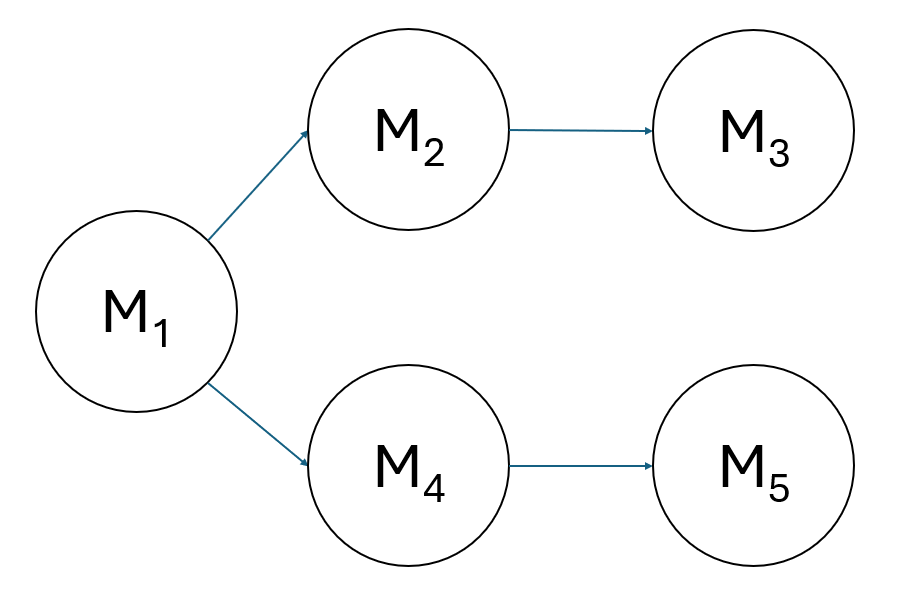
\includegraphics[width=0.7\textwidth]{immagini/3 - Brute Force e Algoritmi Greedy/Idee Greedy/Esempio Introduttivo.png}
	\caption{Percorso con piazze (cerchi) e strade (frecce). Con $M_i$ sono indicate le monete presenti in ogni piazza}
	\label{fig:Brute-Force-Algoritmi-Greedy:Idee-Greedy:Esempio-Introduttivo}
\end{figure}

L'approccio \textbf{Brute Force} consiste nel percorrere tutte le strade e, quindi, valutare il massimo tra:

\begin{itemize}
	\item $M_1 + M_2 + M_3$
	\item $M_1 + M_4 + M_5$
\end{itemize}

Ciò garantisce la correttezza della soluzione pagando in termini di complessità computazionale: al crescere delle possibili strade, l'algoritmo diventa insostenibile in termini di costo.

\medskip

Un approccio \textbf{Greedy}, invece, consiste nel prendere, ad ogni piazza, la scelta immediatamente più conveniente, cioè seguire la strada che conduce alla piazza con il maggior numero di monete tra quelle disponibili.
In altre parole, a ogni nodo del grafo, si seleziona localmente il percorso che massimizza la quantità di monete raccolte in quel passo, senza considerare tutte le possibili combinazioni future.

Con riferimento alla figura \ref{fig:Brute-Force-Algoritmi-Greedy:Idee-Greedy:Esempio-Introduttivo}, partendo dalla piazza $M_1$, la scelta greedy consiste nel confrontare le piazze raggiungibili ($M_2$ e $M_4$) e scegliere immediatamente quella con il maggior numero di monete. 
Successivamente, si ripete lo stesso criterio per la piazza successiva fino a raggiungere una piazza terminale o senza uscite disponibili.

Come detto, l'approccio si concretizza nel fare la scelta migliore \emph{localmente}, senza considerare le conseguenze future.



Questo metodo è computazionalmente efficiente, in quanto richiede solo di confrontare i valori locali delle piazze accessibili in ogni passo. 
Tuttavia, \emph{non sempre garantisce il massimo globale}, poiché una scelta ottimale locale potrebbe portare a un percorso complessivamente subottimale. 
Per questo motivo, la strategia greedy va applicata solo quando il problema possiede una struttura che assicuri la correttezza delle scelte locali rispetto alla soluzione globale, oppure come heuristica rapida in problemi di grandi dimensioni.
A tal proposito, in figura \ref{fig:Brute-Force-Algoritmi-Greedy:Idee-Greedy:Controesempio-Introduttivo} è riportato un controesempio che smonta la scelta greedy sopra proposta.

\begin{figure}[h!]
	\centering
	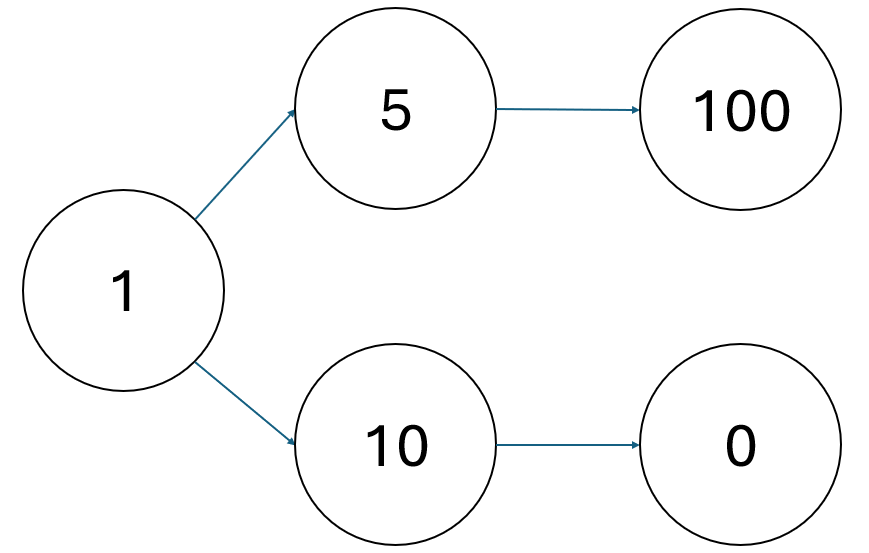
\includegraphics[width=0.7\textwidth]{immagini/3 - Brute Force e Algoritmi Greedy/Idee Greedy/Controesempio Introduttivo.png}
	\caption{Controesempio: scegliendo al primo passo la piazza che garantisce il massimo immediato (10 monete), il percorso totale raccoglie solo 11 monete, mentre scegliendo l'altra strada si potrebbero raccogliere 106 monete. Questo evidenzia come la scelta greedy locale possa portare a un risultato subottimale.}
	\label{fig:Brute-Force-Algoritmi-Greedy:Idee-Greedy:Controesempio-Introduttivo}
\end{figure}






\subsection{Calcolatrice Rotta}
\label{problema:greedy:Calcolatrice-Rotta}

\href{https://training.olinfo.it/task/terry/calcolatrice}{Link al problema}

\bigskip

Francesco ha fatto cadere la sua calcolatrice, e ora non funziona più come dovrebbe!  
Gli unici tasti funzionanti sono il \( - \), il \( \times \), l'\(1\) e il \(2\).  

Per utilizzare la calcolatrice è costretto a partire dal numero \(1\) o dal numero \(2\) (premendo il tasto corrispondente) e applicare zero o più volte una delle \(4\) possibili operazioni funzionanti:

\begin{itemize}
	\item sottrarre \(1\)
	\item sottrarre \(2\)
	\item moltiplicare per \(1\)
	\item moltiplicare per \(2\)
\end{itemize}

Per fare uno scherzo ai suoi amici, vorrebbe raggiungere sulla calcolatrice il numero \(N\).  
Quante operazioni deve fare al minimo per farlo?

\medskip

\noindent \textbf{Nota:} \emph{premere il tasto \(1\) o \(2\) all'inizio conta come un'operazione, inoltre la calcolatrice è danneggiata quindi Francesco è costretto a partire sempre da \(1\) o \(2\) (non può ad esempio premere \(2\) e poi \(1\) per partire dal numero \(21\)) e le uniche operazioni ammesse sono quelle precedentemente elencate (non può per esempio moltiplicare o sottrarre \(12\) o \(21\)).}


\bigskip
\noindent \textbf{Idea (greedy):}








